\subsection{Analisi}
\textit{Periodo: dal 05-11-2020 al 11-01-2021}\\
L'inizio del periodo di questa fase comincia con presentazione dei capitolati e la fine coincide con la data di consegna dei documenti relativi alla revisione dei requisiti.
%Precondizioni:
%\begin{itemize}
%\item formazione del gruppo;
%\item presentazione dei capitolati d'appalto.
%\end{itemize}
%Postcondizioni:
%\begin{itemize}
%\item scelta del nome e del logo del gruppo;
%\item creazione della mail e di una repository per la documentazione;
%\item scelta del capitolato per cui si vuole concorrere;
%\item redazione dei documenti d'ingresso alla RR\glo{};
%\item verifica e approvazione di quanto redatto. 
%\end{itemize}
\subsubsection{Attività}
Questa fase è composta da sette attività che corrispondono ai documenti prodotti:
\begin{itemize}
\item \textbf{\SdF}: viene effettuato uno studio dei capitolati proposti, analizzandone aspetti positivi e negativi al fine di identificare il capitolato per cui concorrere. Questa attività è bloccante per l'\AdR ;
\item \textbf{\NdP}: vengono definite tutte le norme che il gruppo \Gruppo seguirà durante lo sviluppo dell'intero progetto;
\item \textbf{\PdP}: il presente documento, in cui le attività, i compiti\glo{} e le risorse precedentemente analizzate vengono distribuite tra i membri del team \Gruppo{}; presenta il calcolo preventivo per la realizzazione del progetto;
\item \textbf{\AdR}: vengono studiati ed analizzati i requisiti del capitolato\glo{} scelto nello \SdF;
\item \textbf{\PdQ}: si espongono i metodi necessari e scelti a garantire la qualità del prodotto;
\item \textbf{\Glossario}: vengono definiti in modo conciso i termini che possono risultare ambigui durante lo svolgimento del progetto;
\item \textbf{Lettera di Presentazione}: breve documento in cui il gruppo \Gruppo{} si candida come fornitore del prodotto software richiesto.
\end{itemize}
\subsubsection{Periodi}
La pianificazione di questa fase è stata organizzata nei seguenti periodo:
\begin{itemize}
\item \textbf{05-11-2020 - 04-12-2020}: Scelta del nome e del logo del gruppo, creazione della mail di riferimento e individuazione degli strumenti per la comunicazione interna. Discussione dei capitolati proposti per individuare quello preferito dal gruppo e inizio della stesura dello \SdF{} ; iniziato anche il \Glossario \\Il 10-12-2020 il gruppo ha fissato una milestone\glo{} per la conclusione dello \SdF{} e la scelta del capitolato.\\Stesi i verbali interni relativi alle riunioni in questa fase.
\item \textbf{05-12-2020 - 22-12-2020}: Stesura delle \NdP{} e del \PdP{} con l'esposizione della pianificazione del lavoro da svolgere nel corso del progetto e la suddivisione dei ruoli tra i membri del gruppo. Iniziata inoltre la stesura dell'\AdR{}.\\Il 22-12-2020 il gruppo ha fissato una milestone per verificare che il documento \NdP{} sia completato correttamente e valutare come distribuire eventuali ritardi.\\Stesi i verbali interni relativi alle riunioni in questa fase.
\item \textbf{23-12-2020 - 05-01-2020}: Il gruppo si dedica all'\AdR{} e al contempo inizia la stesura del \PdQ{}, con la seguente esposizione dei criteri di valutazione della qualità scelti dal gruppo e le rispettive metriche\glo{} di calcolo.\\Il 05-01-2020 il gruppo fissa un'ulteriore milestone per verificare che tutti i documenti siano stati completati correttamente e valutare come distribuire eventuali ritardi.\\Continuano le attività di verifica incrementale per i documenti in corso di stesura.\\Stesi i verbali interni relativi alle riunioni in questa fase.
\item \textbf{06-01-2020 - 11-01-2020}: Si svolge attività di verifica su tutti i documenti, si completano eventualmente documenti in ritardo. Si uniformano tutti i documenti stando alle regole stabilite nelle \NdP{}. Si scrive inoltre la Lettera di Presentazione.\\Stesi i verbali interni relativi alle riunioni in questa fase.
\end{itemize}
\subsubsection{Diagramma di Gantt: Analisi}
\begin{center}
	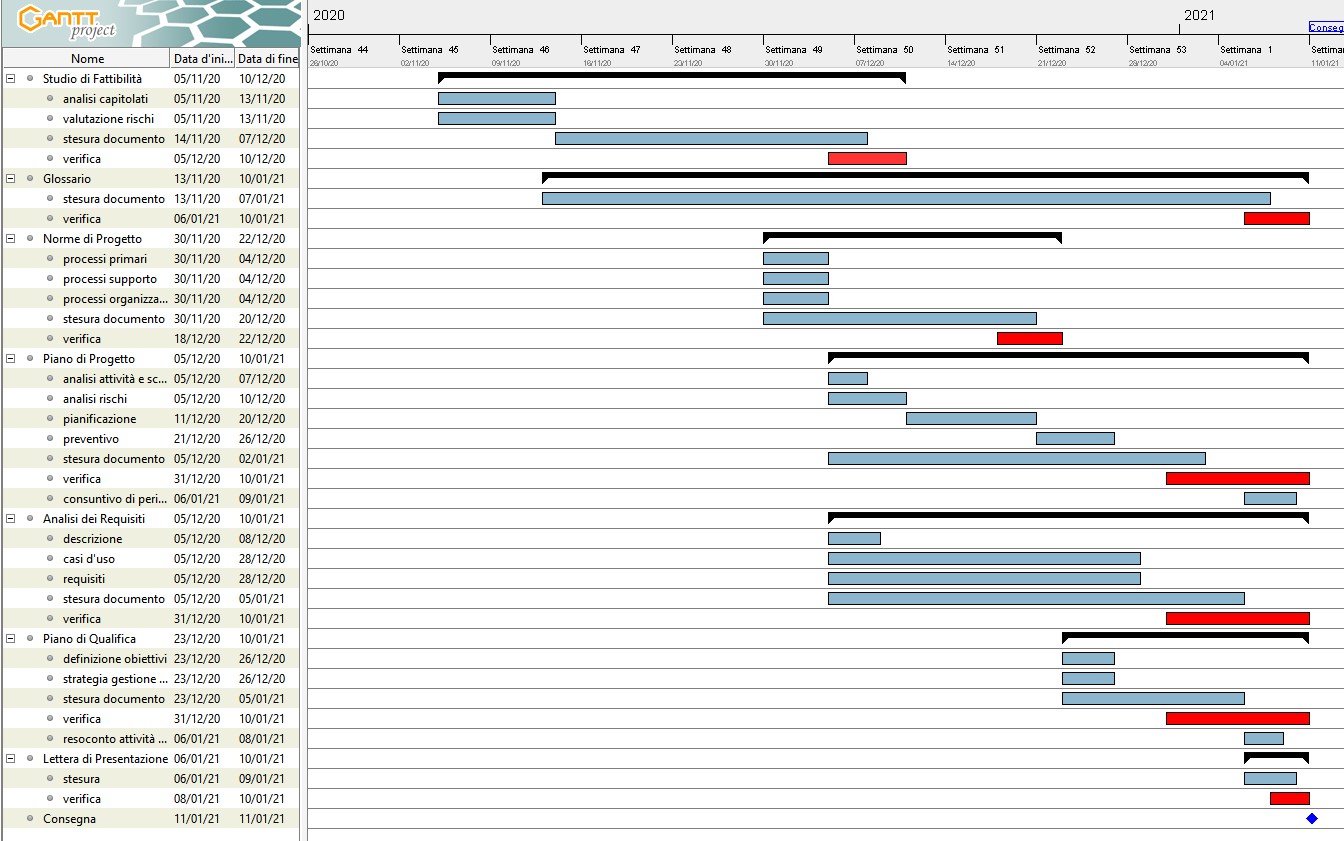
\includegraphics[scale=0.45]{img/gant-analisi.PNG}
	\textbf{Figura 1}: Diagramma di Gantt dell'attività di Analisi
\end{center}